\subsection{Questão de Investigação 2}
Na primeira questão, após serem analisados os dados das taxas de cobertura dos testes da segunda e da quarta semana, observou-se que segundo esses dados, a taxa de cobertura da segunda para a quarta semana diminuiu, e afirmou-se se provavelmente isso aconteceu pois havia mais código para testar, portanto para esta questão de investigação vai-se \textbf{verificar se houve um aumento de linhas de código totais (M18), e se elas estão correlacionadas com a taxa de cobertura dos testes (M24)}

Para verificar se houve um aumento no número de linhas de código totais, começou-se por separar o número de linhas de código escritas na segunda, terceira e quarta semana e escreveu-se um sumário para cada uma e um boxplot para estudar os dados das três amostras, não serão estudadas as linhas de código totais da primeira semana, pois, como ainda não era preciso escrever código para o trabalho de Engenharia de Software II, a maior parte dos grupos deixou esse campo em branco.

\begin{figure}
    \centering
    \label{fig:sumarryLinhasSemana2}
    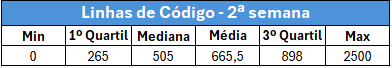
\includegraphics[width=0.5\linewidth]{imagens//questao2/sumarryLinhasSemana2.png}
    \caption{Sumário das linhas de código totais da segunda semana}
    \label{fig:sumarryLinhasSemana2}
\end{figure}

\begin{figure}
    \centering
    \label{fig:sumarryLinhasSemana3}
    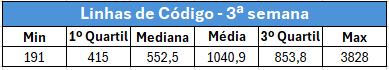
\includegraphics[width=0.5\linewidth]{imagens//questao2/sumarryLinhasSemana3.png}
    \caption{Sumário das linhas de código totais da terceira semana}
    \label{fig:sumarryLinhasSemana3}
\end{figure}

\begin{figure}
    \centering
    \label{fig:sumarryLinhasSemana4}
    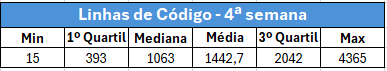
\includegraphics[width=0.5\linewidth]{imagens//questao2/sumarryLinhasSemana4.png}
    \caption{Sumário das linhas de código totais da quarta semana}
\end{figure}

\begin{figure}
    \centering
    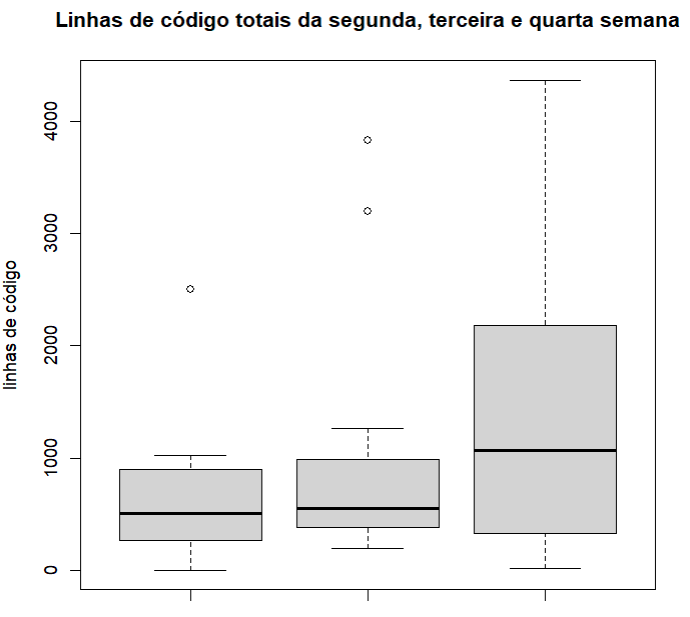
\includegraphics[width=0.5\linewidth]{imagens//questao2/boxplotDas3Semanas.png}
    \caption{BoxPlot das linhas de código totais da 2ª, 3ª e 4ª semana}
    \label{fig:BoxPlotDas3Semanas}
\end{figure}

Como dá para ver pelos sumários das Figuras \ref{fig:sumarryLinhasSemana2}, \ref{fig:sumarryLinhasSemana3} , \ref{fig:sumarryLinhasSemana4},  e sobretudo no boxplot da Figura \ref{fig:BoxPlotDas3Semanas}, consegue-se ver que consoante as semanas passavam, as linhas de código aumentaram.

Ao analisar o sumário das linhas de código na segunda semana (Figura \ref{fig:sumarryLinhasSemana2}), percebemos que o primeiro quartil ($Q_1$) é de 265.0265.0, o segundo quartil ($Q_2$, ou mediana) é de 505.0505.0, e o terceiro quartil ($Q_3$) atinge 898.0898.0. Já na terceira semana (Figura \ref{fig:sumarryLinhasSemana3}), consegue-se ver que houve um aumento significativo nos quartis, com $Q_1=415.0$, $Q_2=552.5$, e $Q_3=853.8$. No final, na quarta semana (Figura \ref{fig:sumarryLinhasSemana4}), os valores continuam a crescer com os quartis $Q_1=393.5$, $Q_2=1063.0$, e $Q_3=2042.0$.

Estas observações são confirmadas visualmente com o boxplot da Figura \ref {fig:BoxPlotDas3Semanas} , onde é possível perceber uma tendência no aumento das linhas de código ao longo das semanas. Este comportamento ascendente sugere que o desenvolvimento de código tornou-se mais extenso à medida que o projeto avançava, possibilitando uma correlação entre o tempo e a complexidade do código.

No entanto, estes dados refletem apenas as medidas de localização das amostras, não representado os valores reais da população, portanto vai ter de se fazer mais testes para verificar se houve mesmo um aumento das linhas de código totais. Para fazer esse estudo, decidiu-se fazer um teste de ANOVA, pois, ele permite comparar as médias populacionais de mais de dois grupos, no entanto, para usar esse teste é preciso saber se as amostras seguem uma distribuição normal, para isso, vai-se fazer o teste de shapiro para as três amostras.

\begin{figure}
    \centering
    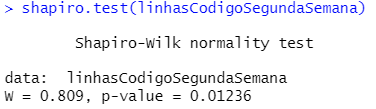
\includegraphics[width=0.5\linewidth]{imagens//questao2/testeShapiroLinhasSegundaSemana.png}
    \caption{Teste de normalidade aos dados das linhas de código da segunda semana}
    \label{fig:shapiroTesteSemana2Linhas}
\end{figure}

\begin{figure}
    \centering
    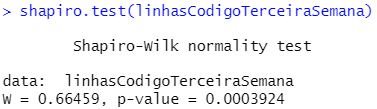
\includegraphics[width=0.5\linewidth]{imagens//questao2/testeShapiroLinhasTerceiraSemana.png}
    \caption{Teste de normalidade aos dados das linhas de código da terceira semana}
    \label{fig:shapiroTesteSemana3Linhas}
\end{figure}

 \begin{figure}
     \centering
     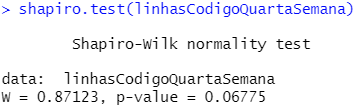
\includegraphics[width=0.5\linewidth]{imagens//questao2/testeShapiroLinhasQuartaSemana.png}
     \caption{Teste de normalidade aos dados das linhas de código da quarta semana}
     \label{fig:shapiroTesteSemana4Linhas}
 \end{figure}

\begin{center}
    H0: As linhas de código totais da semana i seguem uma distribuição normal
    \newline
    vs:
    \newline
    H1: As linhas de código totais da semana i não seguem uma distribuição normal
    \newline
\end{center}
$i \in \{2, 3, 4\}$


 Nas Figuras \ref{fig:shapiroTesteSemana2Linhas} e \ref{fig:shapiroTesteSemana3Linhas}, consegue-se ver que o p-value (0.01236 para a segunda semana e 0.0003924 para a terceira semana) é menor que o nível de significância estabelecido de 5\%, ´rejeitando a hipótese nula, existindo evidências estatísticas que os dados das linhas de código da segunda e terceira semana não seguem uma distribuição normal. No entanto, na Figura \ref{fig:shapiroTesteSemana4Linhas}, o p-value (0.06775) é maior que o nível de significância estabelecido de 5\%, não rejeitando a hipótese nula, existindo evidências estatísticas que os dados das linhas de código da quarta semana seguem uma distribuição normal.
 Como apenas os dados da quarta semana seguem uma distribuição normal, já não dá para usar um teste de ANOVA, assim, vai ter de ser substituído por um teste não paramétrico, sendo o teste escolhido o de Kruskal-Wallis, visto que as amostras são independentes, nele é testado a igualdade das medianas de todos os grupos, ao contrário do teste de ANOVA que testava as médias. Caso as amostras fossem emparelhadas, ter-se-ia de usar um teste de Friedman.

 \begin{center}
    $H0: {\eta}_{semana2} = {\eta}_{semana3} = {\eta}_{semana4}  \hspace{1cm}$
    \newline
    vs:
    \newline
    $h1: {\eta}_{semana2} \ne {\eta}_{semana3} \ne {\eta}_{semana4}$
    \newline
\end{center}

\[ H0: {\eta}_{semana2} = {\eta}_{semana3} = {\eta}_{semana4}  \hspace{1cm} vs: \hspace{1cm} h1: {\eta}_{semana2} \ne {\eta}_{semana3} \ne {\eta}_{semana4} \] \begin{figure}
    \centering
    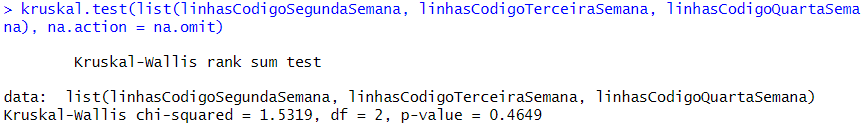
\includegraphics[width=0.5\linewidth]{imagens//questao2/testeKruskaWallis.png}
    \caption{ Teste de Kruskall-Wallis para comparar as medianas da segunda, terceira e quarta semana}
    \label{fig:kruskalWallisTestPergunta2}
\end{figure}

A partir do output da Figura \ref{fig:kruskalWallisTestPergunta2}, consegue-se ver que o p-value (0.4649) é maior que o nível de significância estabelecido de 5\%, logo a hipótese nula não é rejeitada, verificando-se que ao contrário do que foi visto a partir da análise das amostras, existem evidências estatísticas que as medianas das linhas de código das três semanas são estatisticamente iguais.

%---------------------------------------daria para fazer uma nova pergunta com o que vem para a frente
Após se verificar que não houve aumento significativo das linhas de código totais, vai-se confirmar se estas, correlacionam com a taxa de cobertura dos testes, e provar se a afirmação da primeira pergunta é válida.

Para poder estudar a validade da afirmação dessa afirmação, vai ter de se fazer um teste de correlação para saber se os dados das linhas de código totais estão correlacionados com os dados da taxa de cobertura dos testes, mas antes, é preciso fazer um teste de normalidade às duas amostras para saber se se vai usar um teste de correlação de Pearson ou um teste de correlação de Spearman.

Nos dados a cerca das linhas linhas de código totais e da taxa de cobertura dos testes, foram ignorados os dados da primeira semana, pois nessa altura ainda não era preciso escrever código, contendo muito pouca informação, e a escassa informação que tem pode não ser credível.


\begin{figure}
    \centering
    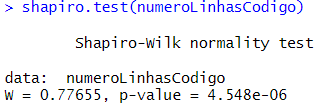
\includegraphics[width=0.5\linewidth]{imagens//questao2/shapiroTestLinhasDeCodigoParaCorrelacao.png}
    \caption{Teste de normalidade de Shapiro-Wilk para os dados sobre o numero de linhas de código totais}
    \label{fig:ShairoTestLinhasParaCorrelacao}
\end{figure}
\begin{figure}
    \centering
    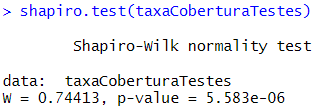
\includegraphics[width=0.5\linewidth]{imagens//questao2/ShapiroTestTaxaCoberturaParaCorrelacao.png}
    \caption{Teste de normalidade de Shapiro-Wilk para os dados sobre a taxa de cobertura dos testes}
    \label{fig:ShairoTestTaxaCoverturaParaCorrelacao}
\end{figure}

\begin{center}
    H0: As linhas de código totais seguem uma distribuição normal
    \newline
    vs:
    \newline
    H1:As linhas de código totais não seguem uma distribuição normal
    \newline
\end{center}
\newline
\begin{center}
    H0: A taxa de cobertura dos testes seguem uma distribuição normal
    \newline
    vs:
    \newline
    H1:A taxa de cobertura dos testes não seguem uma distribuição normal
    \newline
\end{center}

Como dá para ver nas Figuras \ref{fig:ShairoTestLinhasParaCorrelacao} e \ref{fig:ShairoTestTaxaCoverturaParaCorrelacao}, os p-values dos dois testes ($4.548 * 10^{-6}$ e $5.583 * 10^{-6}$) são menores que o nível de significância estabelecido de 5\%, rejeitando a hipótese nula, comprovando que existem evidências estatísticas que os dados do número de linhas de código totais e da taxa de cobertura dos testes não seguem uma distribuição normal, assim será preciso usar um teste de correlação de Spearman, pois este é uma alternativa não paramétrica ao teste de Pearson, que precisa que os dados sigam uma distribuição normal.

\begin{figure}
    \centering
    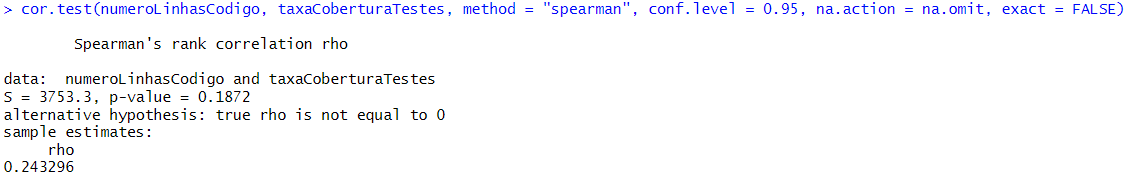
\includegraphics[width=0.5\linewidth]{imagens//questao2/pergunta2TesteCorrelacaoSpearman.png}
    \caption{Teste de correlação de Spearman para os dados das linhas de código totais e para a taxa de cobertura dos testes}
    \label{fig:TesteCorrelacaoSpearmanPergunta2}
\end{figure}

\begin{center}
    H0: Coeficiente de correlação é igual a 0
    \newline
    vs:
    \newline
    H1: Coeficiente de correlação é diferente a 0
    \newline
\end{center}


\begin{center}
H0: Coeficiente de correlação é igual a 0 \hspace{1cm} vs: \hspace{1cm} H1: Coeficiente de correlação é diferente a 0
\end{center}

A partir do output da Figura \ref{fig:TesteCorrelacaoSpearmanPergunta2} é possível verificar que o p-value (0.1872) é menor que o nível de significância estabelecido de 5\%, não rejeitando a hipótese nula, existindo evidências estatísticas que o coeficiente de correlação é igual a 0.
O coeficiente de correlação de Spearman, denominado por $\rho $ (rho), é um número que varia entre -1 e +1. Quanto mais próximo dos extremos (-1 ou 1), maior é a força da correlação. Já os valores próximos de 0 implicam em correlações mais fracas ou inexistentes. No output apresentado, é possível ver que o coeficiente de correlação (0.243296) está muito próximo de zero.

Outra forma de ver se a correlação entre os dados é através de um gráfico de dispersão, assim é possível identificar padrões e tendências nos dados, servindo como guia visual entre a relação entre as duas variáveis.
Na Figura \ref{fig:ScatterPlotPergunta2}, é apresentado um gráfico de dispersão que representa os pontos correspondentes ao número de linhas de código totais no eixo x e à taxa de cobertura dos testes no eixo y., onde cada ponto no gráfico representa uma observação individual. A inclinação geral da dispersão de pontos pode indicar a direção da relação entre as variáveis: se os pontos estão inclinados para cima, sugere uma correlação positiva, enquanto uma inclinação para baixo indica uma correlação negativa.

A adição da linha de regressão linear (representada em vermelho) ajuda a destacar a tendência geral dos dados. No entanto, segundo o resultado do teste de correlação de Spearman, não foi encontrada uma correlação significativa entre essas variáveis. O gráfico de dispersão, juntamente com a análise estatística, proporciona uma abordagem abrangente para a compreensão da relação entre o número de linhas de código e a taxa de cobertura dos testes.

 \begin{figure}
     \centering
     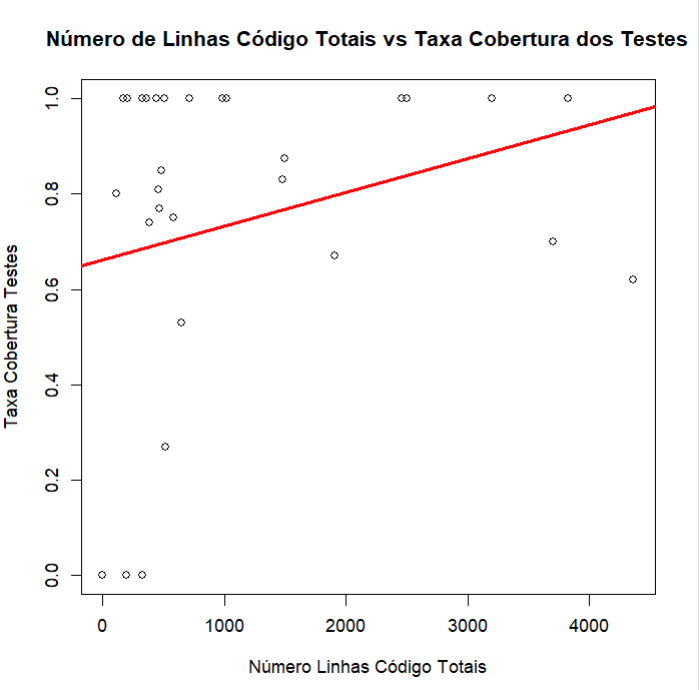
\includegraphics[width=0.5\linewidth]{imagens//questao2/scatterPlotCorrelacaoPergunta2.png}
     \caption{Gráfico de dispersão dos dados das linhas de código totais com a taxa de cobertura dos testes}
     \label{fig:ScatterPlotPergunta2}
 \end{figure}

  \textbf{Conclusão:} Com os testes realizados, provou-se que para além de não ter havido uma evolução significativa no número de linhas de código totais no decorrer do projeto de Engenharia de Software II, também se provou que a afirmação feita na primeira pergunta não tem validade, os dados sobre as linhas de código totais e a taxa de cobertura dos testes não estão correlacionados